
%liste des package
\documentclass[12pt]{article}
\usepackage[francais]{babel}
\usepackage[utf8x]{inputenc}
\usepackage{amsmath}
\usepackage{graphicx}
\usepackage[colorinlistoftodos]{todonotes}


\begin{document}

	\begin{titlepage}
		\newcommand{\HRule}{\rule{\linewidth}{0.5mm}} 

		\center 
 		
 		\textsc{\LARGE Polytech Intl}\\[1.5cm] 
		\textsc{\Large IRM 2}\\[0.5cm] 
		\textsc{\large WEB}\\[0.5cm]
		
		%titre
		
		\HRule \\[0.6cm]
		{ \huge \bfseries Catalogue d'images en ligne}\\[0.4cm] 
		\HRule \\[1.5cm]
		
		%nom
		\begin{minipage}{0.4\textwidth}
		\begin{flushleft} \large
		\emph{}\\
		Faysel \textsc{Marsit} % Your name
		\end{flushleft}
		\end{minipage}
		~
		\begin{minipage}{0.4\textwidth}
		\begin{flushright} \large
		\emph{}\\
		Mohamed \textsc{Bouden} % Supervisor's Name
		\end{flushright}
		\end{minipage}\\[2cm]
	
		{\large \today}\\[2cm]
		
		\vfill
		
	
	
	
	\end{titlepage} % fin page de garde


	\section{Introduction}
	Dans le cadre de notre projet web, nous avons choisi la réalisation d’un site internet qui gére la publication des images ,Albums et Auteur.
	
	
	Vous verrez également dans ce projet une application directe des compétences acquises en langages PHP,JAVASCRIPT, HTML et CSS.
	
	
	\subsection{spécification fonctionnelle}


	\begin{itemize}
	\item Ajouter une image / Album / Auteur
	\item Modifier la description de l'image / album / auteur 
	\item Supprimer une image / album / auteur
	\item Visualiser la liste des images / albums / auteurs 
	\item Envoyer une carte postale à un compte mail
	\end{itemize}
	
	
     

   
    
	
	
	
	\newpage
	\section{Analyse}
	Dans cette partie, nous utilisons la modélisation UML pour représenter les spécifications des exigences grâce au diagramme de cas d’utilisation, mais aussi pour analyser le domaine avec le diagramme de classe.
	\subsection{Diagramme de Cas d'Utilisation}
	Les acteurs sont les suivants:
	
	\textbf{L'auteur} :personne qui peut publier des images ,les modifier , les organiser dans des albums  et envoyer des cartes postales par mail
	
	\textbf{L'admin} : personne qui gere les comptes des auteurs  et maintient le site web 
	\vspace{1.5cm}
	
	
	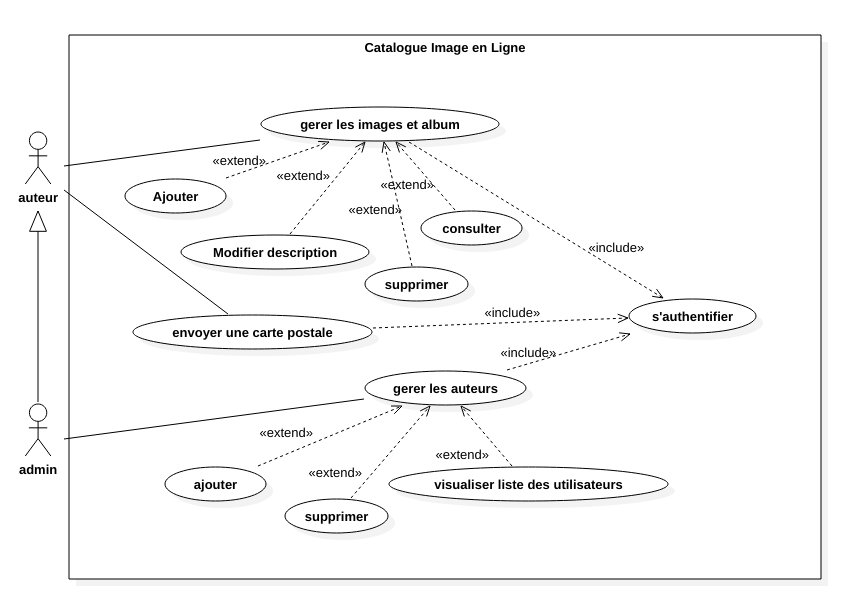
\includegraphics[scale =0.5 ,width=\textwidth]{../usecase.png}
	
	
	\newpage
	\subsection{Conception de Base de donnée}
	
	\vspace{1.5cm}	
	
	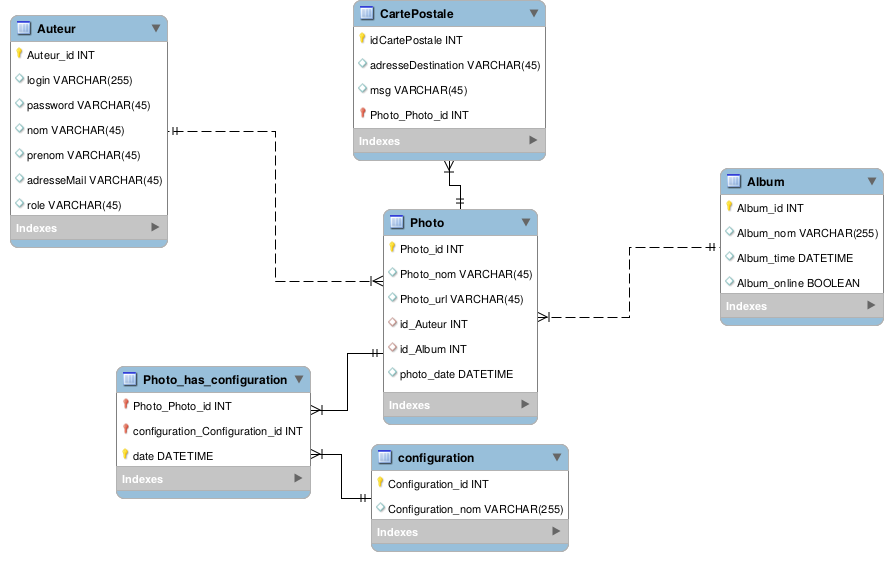
\includegraphics[scale =0.5 ,width=\textwidth]{../base.png}
	
	


\end{document}